\section{Background}\label{sec:bacground}

\subsection{P4}

(This section is adapted from~\cite{budiu-osr17}.)  P4 is a relatively
simple, statically-typed programming language, with a syntax based on
C, designed to express transformations of network packets.

The core abstractions provided by the P4 language are listed in
Figure~\ref{fig:abstractions}.  P4 provides no support for pointers,
dynamic memory allocation, floating-point numbers, or recursive
functions; looping constructs are only allowed within parsers.

\definecolor{grey}{rgb}{0.9, 0.9, 0.9}
\global\mdfdefinestyle{mdstyle}{%
innerleftmargin=.3cm,rightmargin=.3cm,backgroundcolor=grey}
\begin{figure*}[h]
  \begin{mdframed}[style=mdstyle]
    \begin{description}
\item[Headers] describe the format (the set of fields, their ordering
  and sizes) of each header within a network packet.
\item[User-defined metadata] are user-defined data structures
  associated with each packet.
\item[Intrinsic metadata] is information provided or consumed by the
  target, associated with each packet (e.g., the input port where a
  packet has been received, or the output port where a packet has to
  be forwarded).
\item[Parsers] describe the permitted header sequences within received
  packets, how to identify those header sequences, and the headers to
  extract from packets.  Parsers are expressed as state-machines.
\item[Actions] are code fragments that describe how packet header
  fields and metadata are manipulated. Actions may include parameters
  supplied by the control-plane at run time (actions are closures
  created by the control-plane and executed by the data-plane).
\item[Tables] associate user-defined keys with actions.  P4 tables
  generalize traditional switch tables; they can be used to implement
  routing tables, flow lookup tables, access-control lists, and other
  user-defined table types, including complex decisions depending on
  many fields.  At runtime tables behave as match-action
  units~\cite{bosshart-sigcomm13}, processing data in three steps:
  \begin{itemize}
    \item Construct lookup keys from packet fields or computed
      metadata,
    \item Perform lookup in a table populated by the control-plane,
      using the constructed key, and retrieving an action (including
      the associated parameters),
    \item Finally, execute the obtained action, which can modify the
      headers or metadata.
  \end{itemize}
\item[Control] blocks are imperative programs describing the
  data-dependent packet processing including the data-dependent
  sequence of table invocations.
\item[Deparsing] is the construction of outgoing packets from the
  computed headers.
\item[Extern objects] are library constructs that can be manipulated
  by a P4 program through well-defined APIs, but whose internal
  behavior is hardwired (e.g., checksum units) and hence not
  programmable using P4.
\item[Architecture definition:] a set of declarations that describes
  the programmable parts of a network processing device.
    \end{description}
  \end{mdframed}
  \caption{\sl Core abstractions of the P4 programming language.\label{fig:abstractions}}
\end{figure*}

\subsection{P4 Architectures}

P4 allows programs to execute on arbitrary \emph{targets}.  Targets
differ in their functionality, (e.g., a switch has to forward packets,
a network card has to receive or transmit packets, and a firewall has
to block or allow packets), and also in their custom capabilities
(e.g., ASICs may provide associative TCAM memories or custom checksum
computation hardware units, while an FPGA switch may allow users to
implement custom queueing disciplines).  P4 embraces this diversity of
targets and provides some language mechanisms to express it.

\begin{figure}[h]
  \centerline{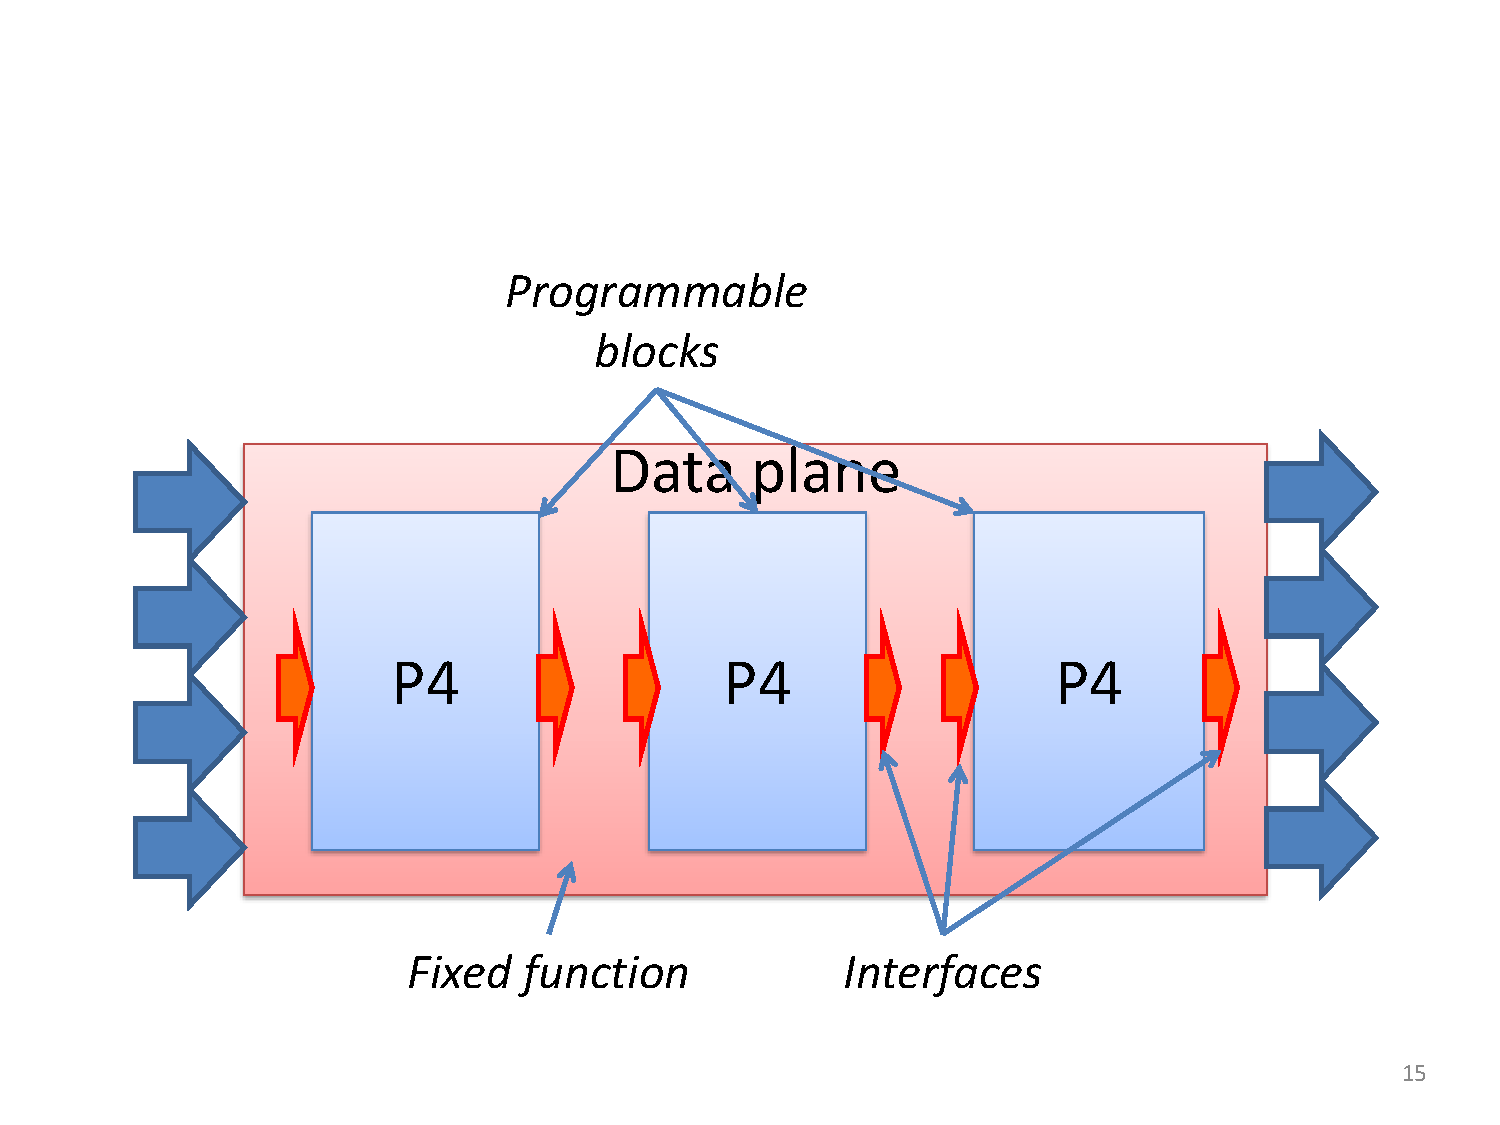
\includegraphics[width=.5\textwidth,clip,trim=1in 0.9in
      .8in 1.8in]{architecture.pdf}}
  \caption{\sl Generic abstract packet-processing engine programmable
    in P4.  The blocks labeled with P4 are programmable in P4; the
    surrounding block is fixed-function
    logic.\label{fig:architecture}}
\end{figure}

Figure~\ref{fig:architecture} is an abstract view of how a P4 program
interacts with the data-plane of a packet-processing engine.  The
data-plane is a fixed-function device that provides several
programmable ``holes''.  The user writes a P4 program to specify the
behavior of each hole.  The target manufacturer describes the
interfaces between the programmable blocks and the surrounding
fixed-function blocks.  These interfaces are target-specific.  Note
that the fixed-function part can be software, hardware, firmware, or a
mixture.

A P4 architecture file is expected to contain declarations of types,
constants, and a description of the control and parser blocks that the
users need to implement.  Section~\ref{sec:ebpf} contains an example
P4 architecture description file.

\subsection{eBPF for network processing}

(This section is adapted from~\cite{p4-ebpf-backend}.)  eBPF is a
acronym that stands for Extended Berkeley Packet Filters. In essence
eBPF is a low-level programming language (similar to machine code);
eBPF programs are traditionally executed by a virtual machine that
resides in the Linux kernel. eBPF programs can be inserted and removed
from a live kernel using dynamic code instrumentation. The main
feature of eBPF programs is their static safety: prior to execution
all eBPF programs have to be validated as being safe, and unsafe
programs cannot be executed. A safe program provably cannot compromise
the machine it is running on:
\begin{itemize}
\item it can only access a restricted memory region (on the local
  stack),
\item it can run only for a limited amount of time; during execution
  it cannot block, sleep or take any locks,
\item it cannot use any kernel resources with the exception of a
  limited set of kernel services which have been specifically
  whitelisted, including operations to manipulate tables (described
  below)
\end{itemize}

\subsubsection{Kernel hooks}

eBPF programs are inserted into the kernel using hooks. There are
several types of hooks available:

\begin{itemize}
\item function entry points can act as hooks; attaching an eBPF
  program to a function foo() will cause the eBPF program to execute
  every time some kernel thread executes foo().

\item eBPF programs can also be attached using the Linux Traffic
  Control (TC) subsystem, in the network packet processing
  datapath. Such programs can be used as TC classifiers and actions.

\item eBPF programs can also be attached to sockets or network
  interfaces. In this case they can be used for processing packets
  that flow through the socket/interface.
\end{itemize}

\subsubsection{eBPF Maps}

The eBPF runtime exposes a bi-directional kernel-userspace data
communication channel, called maps.  eBPF maps are essentially
key-value tables, where keys and values are arbitrary fixed-size
bitstrings. The key width, value width and the maximum number of
entries that can be stored in a map are declared statically, at the
map creation time.

In user-space maps are are exposed as file descriptors. Both user- and
kernel-space programs can manipulate maps by inserting, deleting,
looking up, modifying, and enumerating entries.

In kernel space the keys and values are exposed as pointers to the raw
underlying data stored in the map, whereas in user-space the
pointers point to copies of the data.

\subsubsection{Concurrency}

An important aspect to understand related to eBPF is the execution
model. An eBPF program is triggered by a kernel hook; multiple
instances of the same kernel hook can be running simultaneously on
different cores.

A map may be accessed simultaneously by multiple instances of the same
eBPF program running as separate kernel threads on different cores.
eBPF maps are native kernel objects, and access to the map contents is
protected using the kernel RCU mechanism. This makes access to table
entries safe under concurrent execution; for example, the memory
associated to a value cannot be accidentally freed while an eBPF
program holds a pointer to the respective value.  However, accessing
maps is prone to data races; since eBPF programs cannot use locks,
some of these races often cannot be avoided.

\subsection{XDP: eXpress data path}
An XDP program is similar to other form of eBPF programs, but it attaches
to the very lower networking stack, i.e., the driver layer.
The core idea behind XDP is optimizing cases where relatively simple
decisions can be made about incoming packets. It allows the loading
of a eBPF program into the kernel; that program gets an opportunity
to inspect packets at very low layer before they enter the networking
stack itself. With driver's support, an XDP program can inspect a packet
right after the DMA engine places the packet buffer into main memory.
The initial use case for XDP was to enable the quick dropping of
unwanted packets, but it has been expanded to cover more complicated
packet modifications and packet forwarding.

Similar to other eBPF hook point, XDP program can access maps, and 
it can return one of the following actions;
1) XDP\_DROP simply drop the packet, 2) XDP\_TX results in bouncing
the received packet back out to the same port itt arrived on,
3) XDP\_PASS means the XDP program decides to pass the packet to
the normal network stack, and 4) XDP\_REDIRECT forwards the packet
to another network device.

\subsection{Comparison of P4 and eBPF}

A very thorough evaluation of eBPF for writing networking programs can
be found in~\cite{minao-hspr18}.  P4 and eBPF share many features.
Table~\ref{table:compare} shows a comparison of the high-level
features of both languages.

\begin{table*}[h]
  \footnotesize
  \begin{center}
  \begin{tabular}{|l|l|l|} \hline
    \textbf{Feature} & \textbf{P4} & \textbf{eBPF} \\ \hline \hline
    Targets & ASIC, software, FPGA, NIC & Linux kernel \\ \hline
    Licensing & Apache & GPL \\ \hline
    Tools & Compilers, simulators & LLVM back-end, verifier \\ \hline
    Level & High & Low \\ \hline
    Safe  & Yes & Yes \\ \hline
    Safety & Type system & Verifier \\ \hline
    Resources & Statically allocated & Statically allocated \\ \hline
    Policies & Match-action tables & Key-value eBPF maps (tables) \\ \hline
    Extern helpers & Target-specific & Hook-specific \\ \hline
    Control-plane API & Synthesized by compiler & eBPF maps \\ \hline
    Concurrency & No shared R/W state & Maps are thread-safe \\ \hline
  \end{tabular}
  \caption{Feature comparison between P4 and eBPF.}\label{table:compare}
  \end{center}
\end{table*}

Table~\ref{table:limitations} compares the limitations of P4 and eBPF.
P4 was designed as a language for programming switching devices,
working mostly at levels L2 and L3 of the networking stack; while P4
is finding a use for programming network end-points, e.g., smart NICs,
some end-point functionality cannot be naturally expressed in P4
(e.g., TSO, encryption, deep packet inspection).

Many limitations are shared with eBPF.  We conclude that eBPF is a
suitable language for performing relatively simple packet
filtering/rewriting.  Neither language is good enough to implement a
full end-point networking stack.

\begin{table*}[h]
  \footnotesize
  \begin{center}
  \begin{tabular}{|l|l|l|} \hline
    \textbf{Limitation} & \textbf{P4} & \textbf{eBPF} \\ \hline \hline
    Loops & Parsers & Tail call \\ \hline
    Nested headers & Bounded depth & Bounded depth \\ \hline
    Multicast/broadcast & External & Helpers \\ \hline
    Packet segmentation & No & No \\ \hline
    Packet reassembly &	No & No \\ \hline
    Timers/timeouts/aging & External & No \\ \hline
    Queues & No & No \\ \hline
    Scheduling & No & No \\ \hline
    Data structures & No & No \\ \hline
    Payload processing & No & No \\ \hline
    State & Registers/counters & Maps \\ \hline
    Iterating over packet payload & No & No \\ \hline
    Wildcard matches & Yes & No \\ \hline
    Map writes & Control-plane only & Data-plane and control-plane \\ \hline
    Iteration over map values & Control-plane only & Control-plane only \\ \hline
    Synchronization & No & No \\
    (data/data, data/control) & & \\ \hline
    Execution model & Event-driven & Event-driven \\ \hline
    Resources & Statically allocated & Limited stack and buffer \\ \hline
    Control-plane support & Complex, including remote & Simple \\ \hline
    Safety & Safe & Verifier limited to small programs \\ \hline
    Compiler & Target-dependent & LLVM code not always efficient \\ \hline
  \end{tabular}
  \caption{Limitations comparison between P4 and eBPF.}\label{table:limitations}
  \end{center}
\end{table*}
